\chapter{Przebieg Sprintów}
\par
W niniejszym rozdziale opisane zostały kluczowe funkcjonalności/akcje wykonane w każdym sprincie. Należy mieć na uwadze, że na każdy sprint przypadały też przynajmniej 2 spotkania zespołu będące jednocześnie przeglądem postępów prac jak i planowaniem kolejnych. Szczegółowy proces opisany został w rozdziale "Zarządzanie projektem".
\section{Sprint 0}
\textbf{Czas trwania \gls{sprint}u: 29.10.2025 - 12.11.2025 (2 tygodnie)}
\par
Sprint ten był inicjalizacją prac nad projektem. Pierwszym zadaniem było  zrobienie listy kluczowych funkcjonalności jakie system powinien posiadać. Aby uzuepłnić potencjalne braki zespół stworzył ankietę, która została przekazana potencjalnym uzytkownikom systemu. Po upływie 1 tygodnia od rozesłania ankiety, zbieranie odpowiedzi zostało zakończone. W tym czasie zespół stworzył \gls{POC} systemu do monitorowania statystyk urządzeń tworząc pliki konfiguracyjne kompatybilne z systemem monitorowania Prometheus.
\begin{figure}[H]
    \centering
    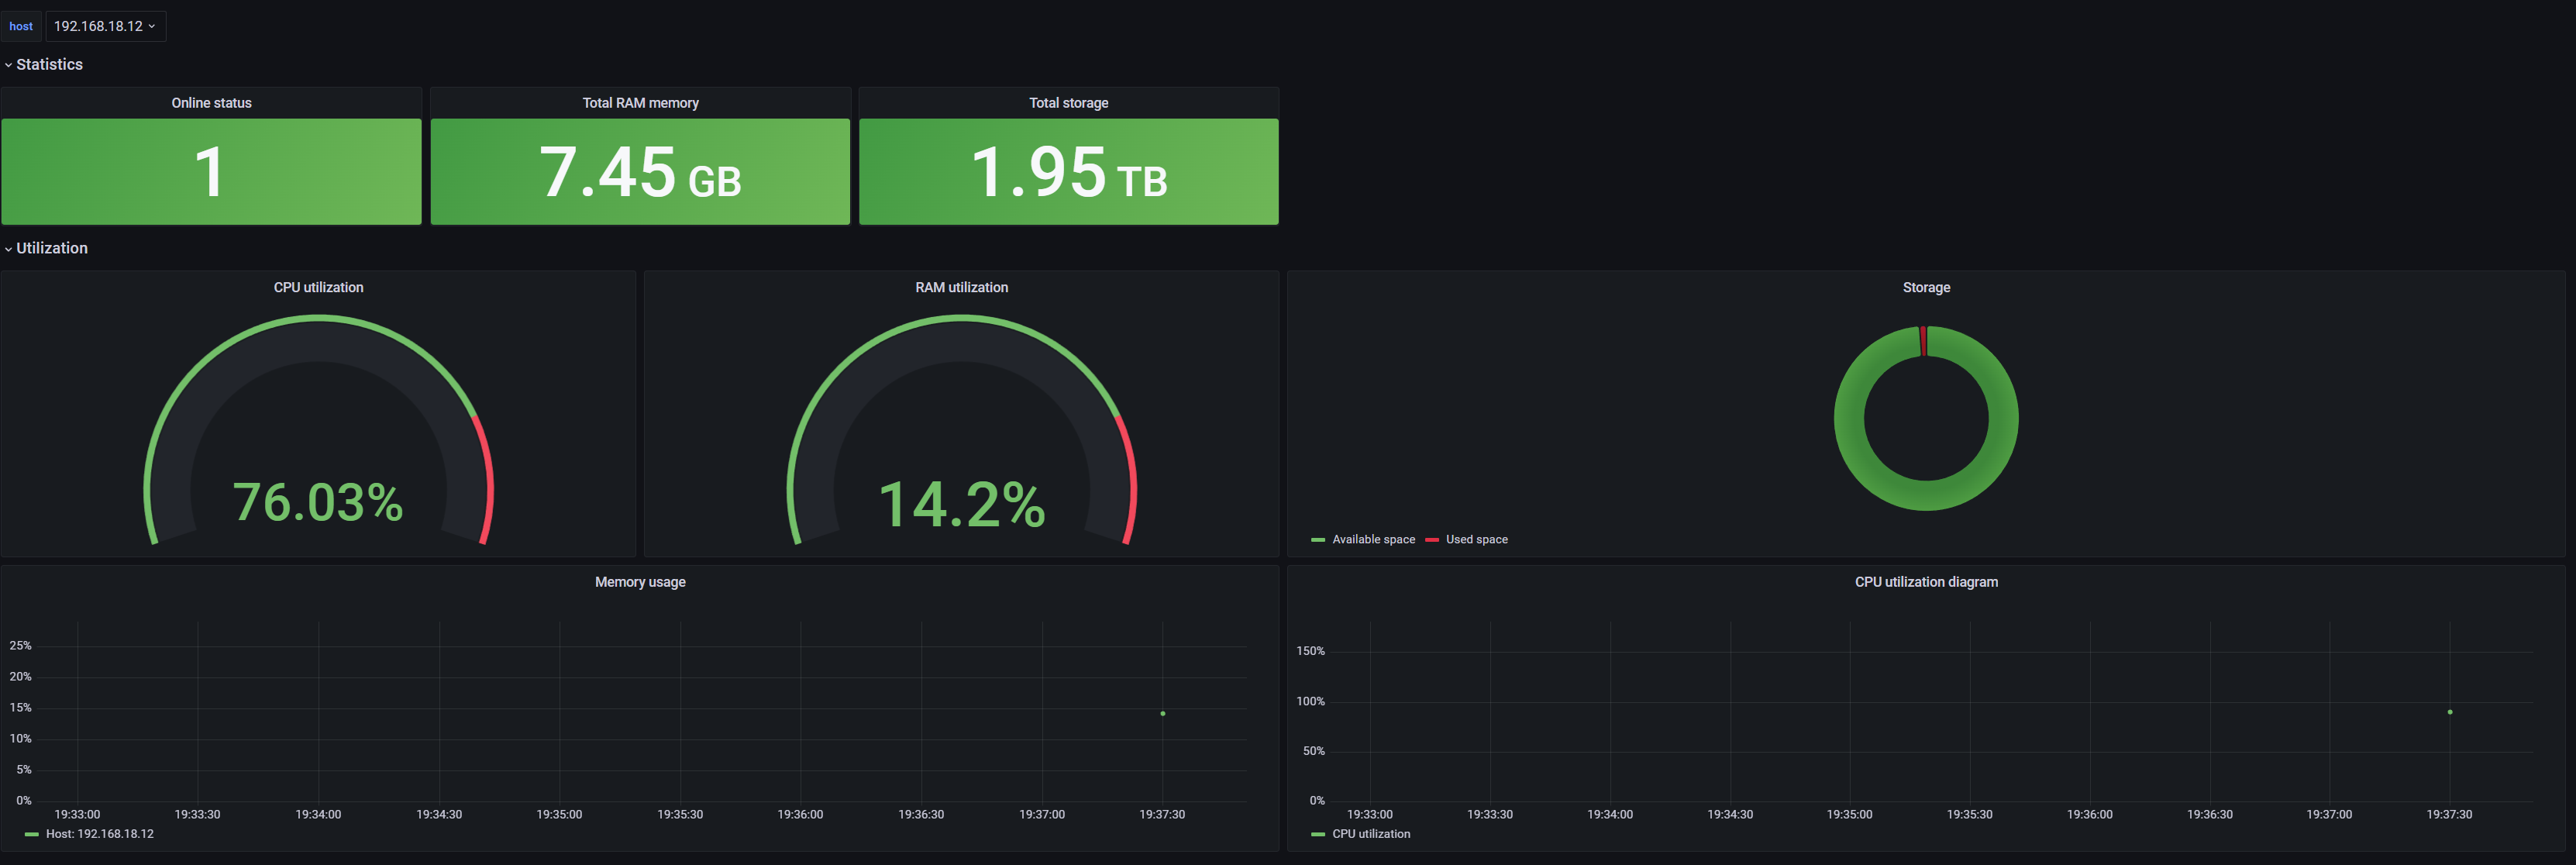
\includegraphics[width=1.0\textwidth]{images/sprint_summary/monitoring_poc.png}
    \caption{Zdjęcie przedstawiające panel monitorowania urządzeń systemu Prometheus (opracowanie własne)}
    \label{img:monitoring_poc}
\end{figure}
repozytoria dla kodu źródłowego: aplikacji oraz tego dokumentu. Repozytoria te zostały skonfigurowane w odpowiedni sposób, by zapobiec wprowadzaniu zmian bezpośrednio do głównej gałęzi, a każda zmiana musiała być poprzedzona \gls{Pull Request}'em, którego zaakceptować musi:
\begin{itemize}
    \item w przypadku kodu źródłowego aplikacji - przynajmniej 1 członek zespołu projektowego,
    \item w przypadku kodu źródłowego dokumentu - cały zespół projektowy.
\end{itemize}
Repozytorium zostało połączone z serwisem Jira w celu sprawniejszego wyszukiwania zmian w kodzie na podstawie zgłoszeń.
\begin{figure}[H]
    \centering
    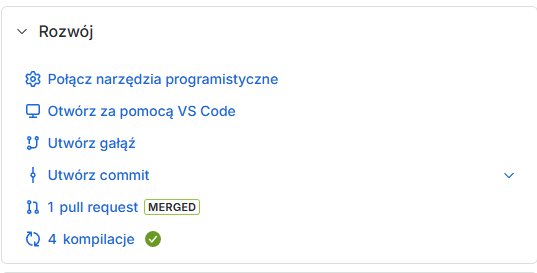
\includegraphics{images/sprint_summary/jira_github_connection.png}
    \caption{Zdjęcie przedstawiające integrację seriwsów GitHub oraz Jira (zrzut erkanu z serwisu Jira, opracowanie własne)}
    \label{img:jira_github_connection}
\end{figure}
Po uzyskaniu odpowiedzi w wyznaczonym czasie, utworzone zostało sprawozdanie z ankiety opisane szczegółowo w punkcie 3.3 . Na jego podstawie wyspecyfikowane zostały wymagania na system, które zostały sklasyfikowane według dwóch wymiarów:
\begin{itemize}
    \item typu wymagania (m.in. dziedzinowe, funkcjonalne, niefunkcjonalne),
    \item przynależności do poszczególnych modułów/obszarów funkcjonalnych (np. Panel Urządzenia, Search Bar).
\end{itemize}
Dzięki temu wytworzone zostały dokumenty takie jak: Karta Projektu, Dokument Założeń Wstępnych czy Specyfikacja Wymagań Systemowych.


\section{Sprint 1}
\textbf{Czas trwania \Gls{sprint}u: 12.11.2025 - 26.11.2025 (2 tygodnie)}
\par
Początkiem \gls{sprint}u utworzony został wstępny model fizyczny bazy danych aplikacji, który wygląda następująco:
\begin{figure}[H]
    \centering
    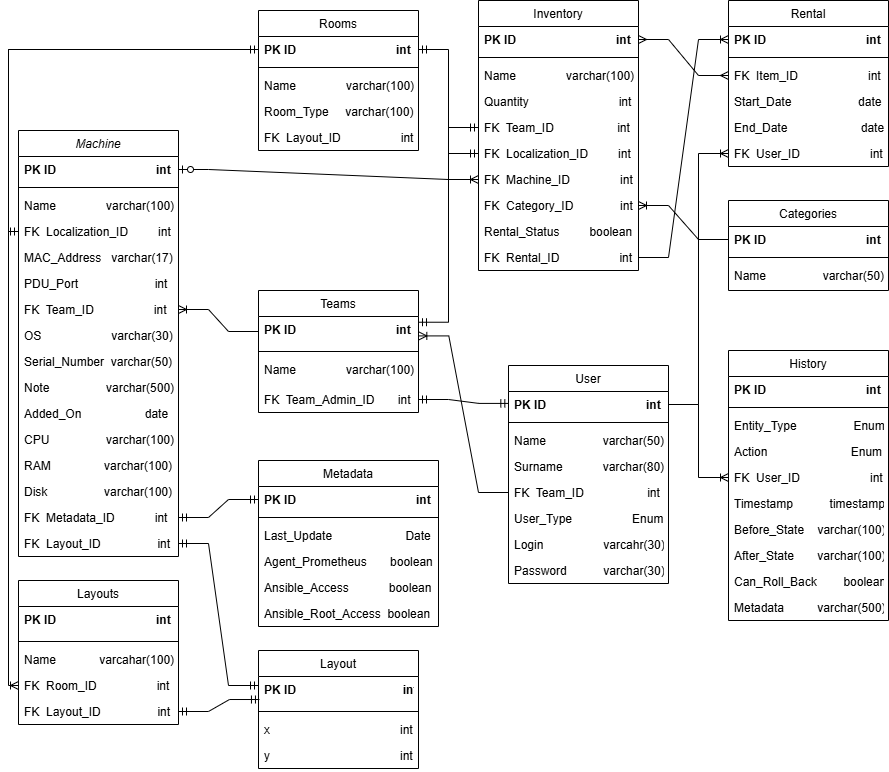
\includegraphics[width=1.0\textwidth]{images/sprint_summary/model_fizyczny_labbyn.png}
    \caption{Wstępny projekt modelu fizycznego bazy danych (opracowanie własne)}
    \label{img:model_fizyczny}
\end{figure}
Model ten posłużył do wstępnej konfiguracji środowiska produkcyjnego oraz umożliwił rozpoczęcie prac nad logiką aplikacji, w ramach której powstało wstępne \gls{API} dla systemu \gls{Prometheus}. Równolegle z jej powstaniem zaimplementowano testy dymne, umożliwiające bieżącą kontrolę poprawności podstawowych funkcjonalności. Ich zastosowanie pozwoliło na szybkie wykrywanie krytycznych błędów po wprowadzanych zmianach.
W celu ujednolicenia wytwarzanego kodu oraz poprawę jego czytelności i utrzymywalności opracowano zbiór wytycznych programistycznych (coding guidelines).
Stworzony został \gls{POC} architektury systemu telemetrii urządzeń w postaci grafu:
\begin{figure}[H]
    \centering
    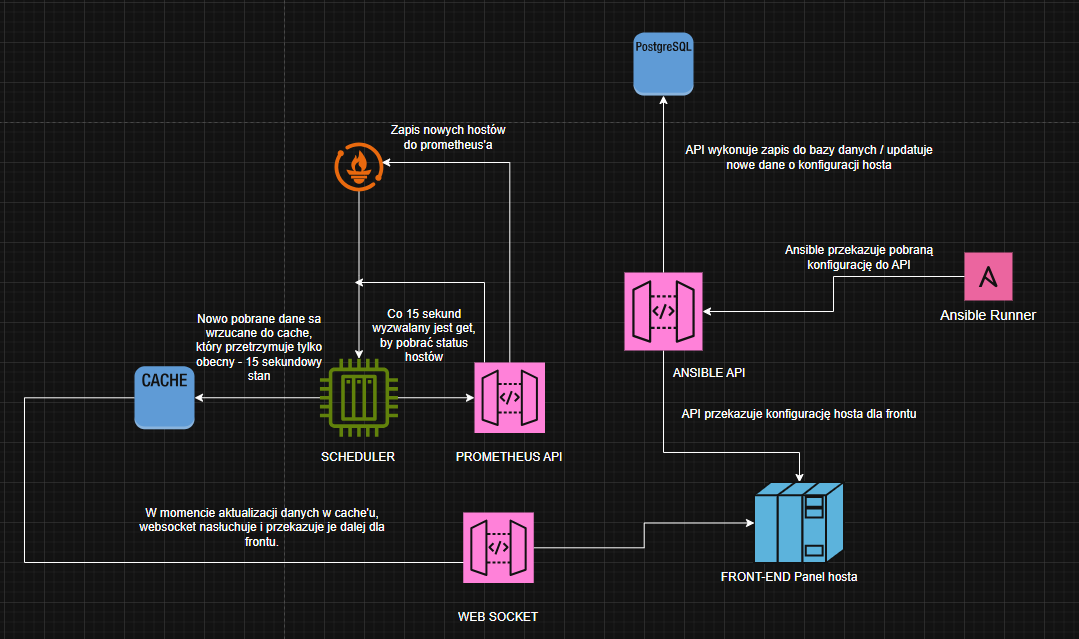
\includegraphics[width=1.0\textwidth]{images/sprint_summary/telemetry_poc.png}
    \caption{POC systemu telemetrii urządzeń (opracowanie własne)}
    \label{img:telemetry_poc}
\end{figure}
Powstała również wersja demonstracyjna aplikacji w celu przedstawienia zespołowi propnowanej wizji artystycznej projektu:
\begin{figure}[H]
    \centering
    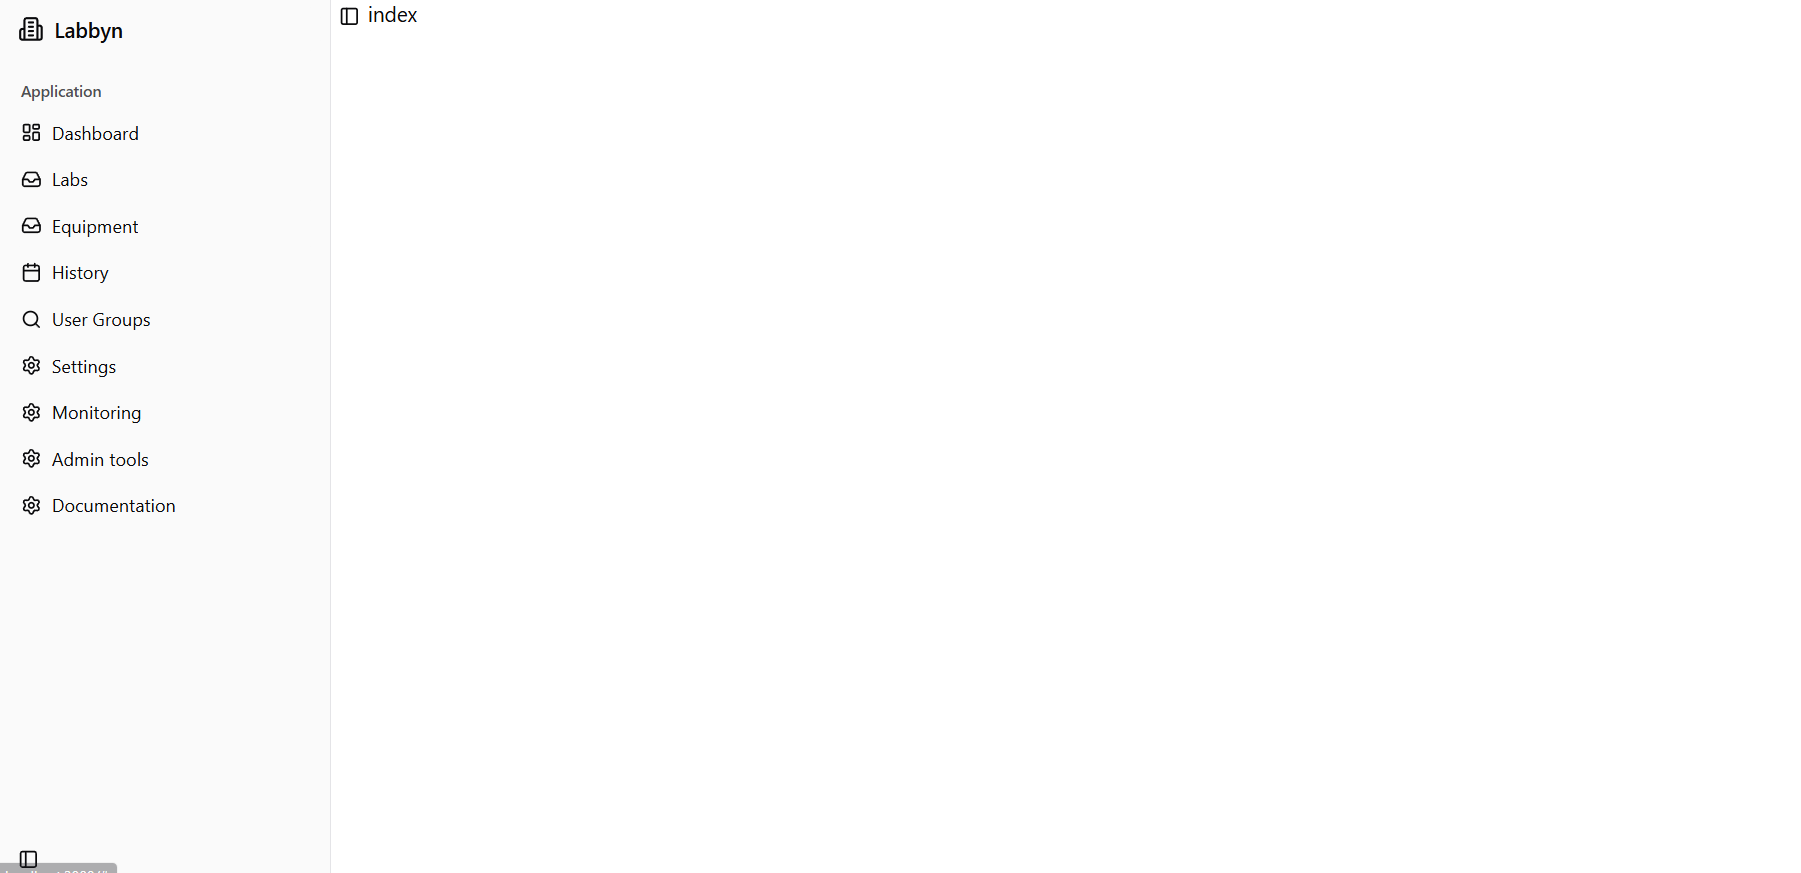
\includegraphics[width=1.0\textwidth]{images/sprint_summary/labbyn_demo_ui.png}
    \caption{Wstępna wersja interfejsu użytkownika (opracowanie własne)}
    \label{img:demo_ui}
\end{figure}
Utworzono podstawowy proces CI/CD wspierający budowanie i testowanie aplikacji, w ramach którego dodano linter jako element workflow CI w GitHubie. Przygotowane zostało również środowisko dewepolerskie umożliwiające obserwowanie zmian w oprogramowaniu w czasie rzeczywistym co zmniejszyło ryzyko powstawania błędów i pozwoliło drastycznie zmniejszyć czas sprawdzania kompatybilności zmian - programista nie był zmuszony budować aplikacji od nowa co było czasochłonne. 

\section{Sprint 2}
\textbf{Czas trwania \Gls{sprint}u: 26.11.2025 - 10.12.2025 (2 tygodnie)}
\par
Podczas tego \gls{sprint}u powstał pierwszy prototyp mapy przestrzennej:
\begin{figure}[H]
    \centering
    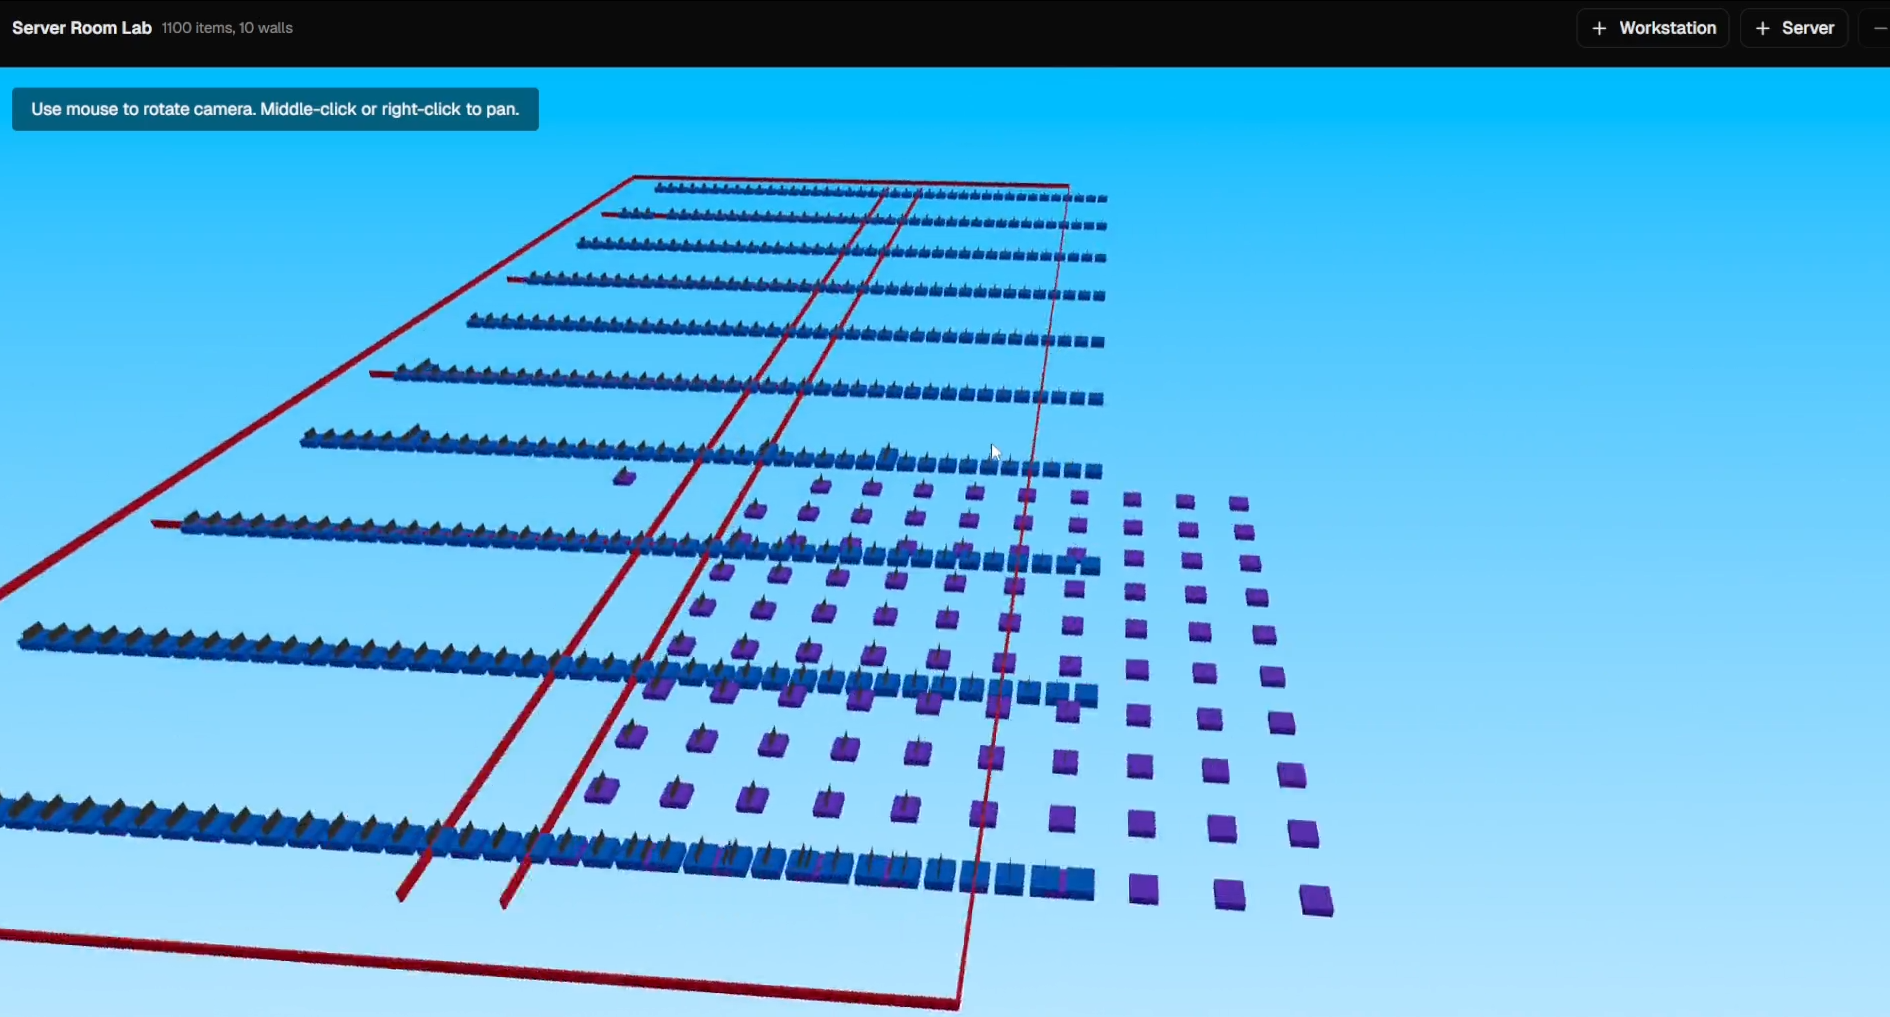
\includegraphics[width=1.0\textwidth]{images/sprint_summary/map_prototype.png}
    \caption{Prototyp mapy przestrzennej laboratorium (opracowanie własne)}
    \label{img:map_prototype}
\end{figure}
Ze względu na brak jednoznacznie zdefiniowanego konceptu wizualnego systemu, przygotowano mockupy w celu ujednolicenia kierunku projeku.
\begin{figure}[H]
    \centering
    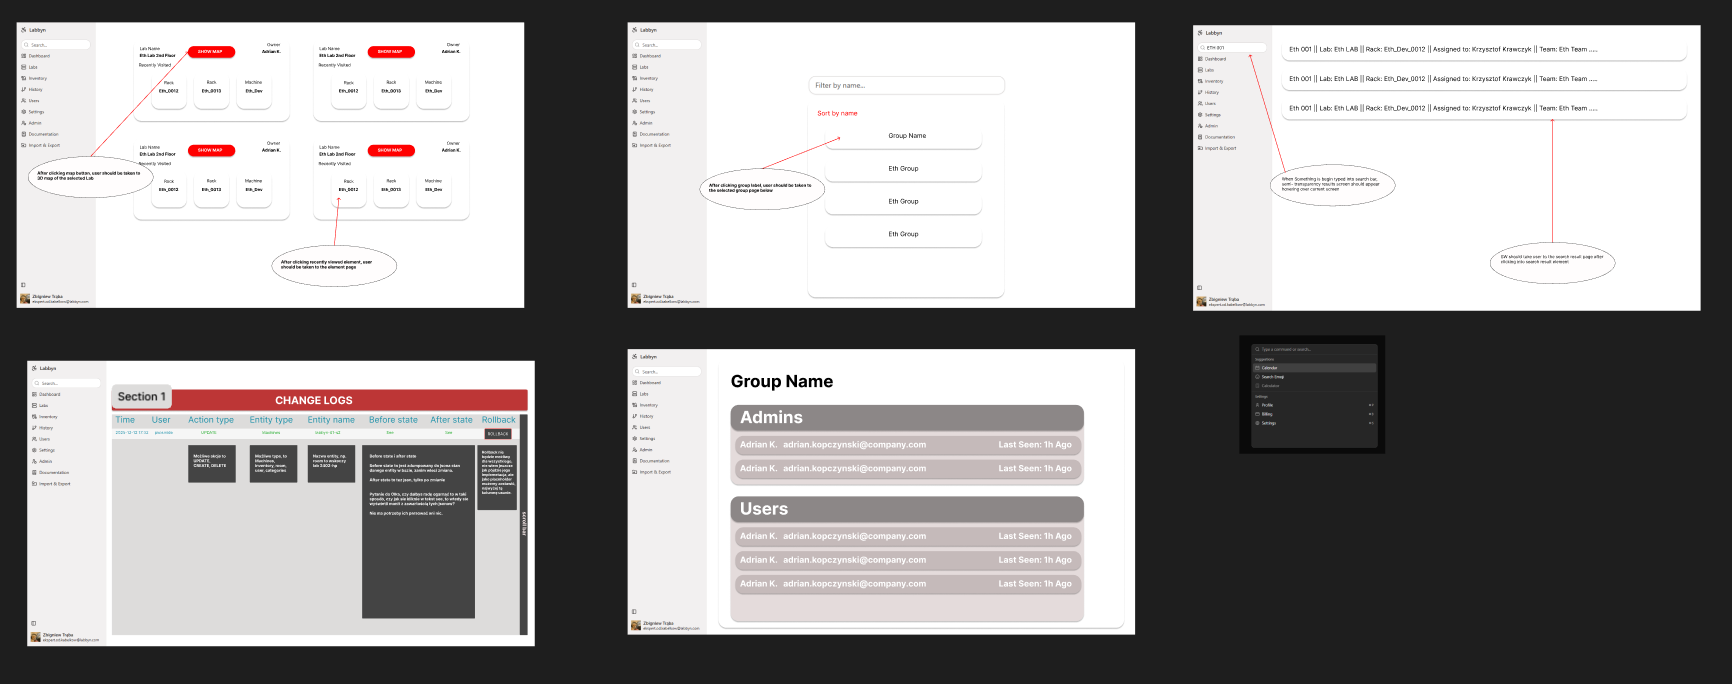
\includegraphics[width=1.0\textwidth]{images/sprint_summary/labbyn_mockups.png}
    \caption{Zdjęcie przedstawiające część mockupów stworzonych dla systemu Labbyn (opracowanie własne)}
    \label{img:labbyn_mockups}
\end{figure}
W ramach implementacji logiki systemu od strony \gls{Backend}u dodano warstwę dostępu do bazy danych z wykrozystaniem \gls{SQL Alchemy} oraz mechanizmy przetwarzania danych jak i obsługi logiki aplikacji.

\section{Sprint 3}
\textbf{Czas trwania \Gls{sprint}u: 10.12.2025 - 07.01.2026 (4 tygodnie)}
\par
Sprint został wydłużony o dwa tygodnie ze względu na okres świąteczny, który ograniczył dostępność zespołu. Podczas tego czasu zaimplementowana została strona logowania użytkownika (bez autoryzacji po stornie \gls{Backend}u), a postronie interfejsu użytkownika, zakładki w systemie na podstawie mockupów wytworzonych w poprzednim sprincie: Labs oraz Documentation.
Implementacja makiet interfejsu użytkownika umożliwiła przeprowadzenie wstępnych testów manualnych, w szczególności w zakresie nawigacji oraz interakcji użytkownika z systemem. Wczesna walidacja systemu pozwoliła na wykrycie błędów w początkowej fazie implementacji, co znacząco uprościło ich eliminację oraz ograniczyło ryzyko propagacji defektów w kolejnych etapach rozwoju.
Zaimplementowane zostało \gls{API} do obsługi \gls{Ansible} wraz z \gls{Playbook}'ami, w ramach którego powstał skrypt, który automatycznie wdraża agenta w celu pobrania konfiguracji sprzętowej. Aby wspomóc testy manualne tej funkcjonalności utworzony został skrypt do tworzenia wirtualnych hostów.
Przygotowana została kontrola dostępu do bazy danych oraz wstępna logika logowania i resetowania hasła użytkownika.
Kluczowym z perspektywy biznesowej było również zaimplementowanie auto-inicjalizacji użytkownika serwisowego w momencie pierwszego zbudowania aplikacji, który umożliwi inicjalny dostęp do aplikacji oraz przeprowadzenie podstawowej konfiguracji, w tym tworzenie kolejnych kont użytkowników.

\section{Sprint 4}
\textbf{Czas trwania \Gls{sprint}u: 07.01.2026 - 28.01.2026 (3 tygodnie)}
\par
Sprint został ponownie wydłużony, tym razem o 1 tydzień, aby jego zakończenie było zbieżne z planowanym zakończeniem etapu 3. co umożliwiło spójne podsumowanie postępów prac.
Zaimplementowano zapis pobranych przez \gls{Ansible} komponentów do bazy danych oraz kolejne zakładki w interfejsie użytkownika: Inventory, Import\&Export, Admin Panel, User, Groups oraz nakładki z funkcją wyszukiwania danych w systemie.
Zdefiniowano plan testów obejmujący scenariusze testowe, środowisko testowe oraz kryteria akceptacji poszczególnych funkcjonalności systemu.
Na potrzeby \gls{MVP} dokonano integracji poszczególnych zakładek interfejsu z \gls{Backend}em, umożliwiając dynamiczne pobieranie i prezentowanie danych z \gls{API}.

\section{Sprint 5}
\textbf{Czas trwania \Gls{sprint}u: 28.01.2026 - 11.02.2026 (2 tygodnie)}
\par
W trakcie realizacji projektu zidentyfikowano niejednoznaczności oraz braki w wymaganiach dotyczących wybranych funkcjonalności (np. proces dodawania nowej maszyny), co utrudniało ich bezpośrednią implementację. Ze względu na ryzyko opóźnienia prac zdecydowano się na opracowanie opisowej logiki biznesowej, która doprecyzowała sposób działania systemu, umożliwiła kontynuację implementacji oraz stanowiła tymczasową specyfikację zachowania systemu. Równocześnie rozpoczęto proces specyfikacji brakujących wymagań w celu zwiększenia kompletności i pokrycia funkcjonalnego systemu.
Podjęto próbę implementacji frameworka do testów end-to-end. Po przeprowadzeniu analizy wartości dodanej, kosztów utrzymania oraz nakładu pracy związanego z integracją z istniejącym procesem CI/CD, zespół zdecydował o rezygnacji z tego rozwiązania.


\section{Sprint 6}
\textbf{Czas trwania \Gls{sprint}u: 11.02.2026 - 25.02.2026 (2 tygodnie)}
\par

\section{Sprint 7}
\textbf{Czas trwania \Gls{sprint}u: 25.02.2026 - 04.03.2026 (1 tygodnie)}
\par

\section{Sprint 8}
\textbf{Czas trwania \Gls{sprint}u: 04.03.2026 - 18.03.2026 (2 tydzień)}
\par

\section{Sprint 9}
\textbf{Czas trwania \Gls{sprint}u: 18.03.2026 - 01.04.2026 (2 tygodnie)}
\par

\section{Sprint 10}
\textbf{Czas trwania \Gls{sprint}u: 01.04.2026 - 15.04.2026 (2 tygodnie)}
\par

\section{Sprint 11}
\textbf{Czas trwania \Gls{sprint}u: 15.04.2026 - 29.04.2026 (2 tygodnie)}
\par
